\documentclass[runningheads]{llncs}
\usepackage{graphicx}
\usepackage{xcolor}
\usepackage{soul,color}
\usepackage{color}
\usepackage{natbib}
\usepackage{listings}
\usepackage{comment}
\usepackage{academicons}
\usepackage[utf8]{inputenc}
\usepackage{amssymb}
\usepackage{pifont}
\usepackage{longtable}
\usepackage{multirow}
\newcommand{\xmark}{\ding{55}}%
\usepackage{xcolor,colortbl}
\definecolor{Gray}{gray}{0.85}
\usepackage[colorinlistoftodos]{todonotes}
\usepackage{academicons}
\usepackage[hidelinks]{hyperref}
\usepackage{rotating}
\usepackage{tikzsymbols}
\usepackage{ragged2e}
%\usepackage{lscape} % to write pages in landscape environment
\usepackage{array, threeparttable} % to add footnotes to the tables
\usepackage[T1]{fontenc}
\usepackage{booktabs}
\usepackage{caption} % to create some space between table caption and table, otherwise there was no space
\captionsetup[table]{skip=5pt}
\hypersetup{pdfstartview={XYZ null null 1.00}}
\newcommand{\orcid}[1]{\href{https://orcid.org/#1}{\textcolor[HTML]{A6CE39}{\aiOrcid}}}
%\setlength\defaultaddspace{0.66ex}

\lstset{escapeinside={<@}{@>}}


\begin{document}

\title{Provenance, Anonymisation and Data Environments: a Unifying Construction  
%1. Data Environment Representation and Limitation of Existing PROV 
%2. Data Environment Representation using Provenance for Anonymisation Decision-Making
%\thanks{Supported by organization x.}
}


\author {Muhammad Aslam Jarwar\inst{1}\orcid{0000-0002-5332-1698}  
\and
Adriane Chapman\inst{2}\orcid{0000-0002-3814-2587} \and 
Mark Elliot\inst{1} \orcid{0000-0002-3142-4493}\and 
Fatemeh Raji\inst{2}\orcid{0000-0001-6130-7135}}
%
\authorrunning{Jarwar et al.}
\newcommand{\titleText}{Provenance, Anonymisation and Data Environments:a Unifying Construction}
\titlerunning{\titleText}
% First names are abbreviated in the running head.
% If there are more than two authors, 'et al.' is used.
%
\institute{University of Manchester, Manchester M13 9PL, UK \\
\email{\{aslam.jarwar, mark.elliot\}@manchester.ac.uk}\\
\and
University of Southampton, Southampton, SO17 1BJ, UK\\
\email{\{adriane.chapman, f.raji\}@soton.ac.uk}}
% 
\maketitle              % typeset the header of the contribution
%
\setcounter{footnote}{0}
\begin{abstract}
The Anonymisation Decision-making Framework (ADF) operationalizes the management of the risk of data exchange between organizations and environments. In its second edition the ADF has increased its emphasis on modelling data flows, highlighting a potential new use for provenance information: to support the  determination of risk of data exchange. We provide a real use case that showcases this functionality. Based on this use case, we identify the requirements for provenance information such that it can be utilized within the ADF, and identify a currently un-met requirement: the modelling of \textit{data environments}. We show how data environments can be implemented within the W3C PROV in three different ways. We analyze each approach for costs and benefits, as well as checking them against a second real use case for completeness. We summarize our findings and suggest ways forward for representing data environments within W3C PROV to underpin the automation of the ADF.

\keywords{Data Environment Representation \and Anonymisation Decision-Making Framework \and Data Provenance \and W3C PROV-DM}
\end{abstract}
%
%
%
%\pagebreak
\section{Introduction}
In the knowledge economy, large amounts of data are collected to support decision-making, policy analytics and service delivery. However, the utility of these data is constrained by the disclosure risks involved in data processing in general and data sharing in particular. One of the tools used to mitigate this risk,  is anonymisation.  The Anonymisation Decision-Marking Framework (ADF) operationalises the processes of functional anonymisation\cite{elliot2018functional}. 
This conceptualization originated in work of the \textit{data environment analysis service}\cite{elliot2010data}; a support system for the 2011 UK census focused on data confidentiality and  disclosure control \cite[e.g.][]{willenborg2012elements,duncan2011concepts,hundepool2012SDC} and in particular re-identification risk assessment \cite [e.g.][]{chen1998, skinner1998estimating,skinner2002measure}. The critical point underlying the concept is that disclosure risk resides not in the data themselves but in the relationship between the data and their environment.  Mackey and Elliot define the data environment as "the set of formal and informal structures, processes, mechanisms and agents that either: (i) act on data; (ii) provide interpretable context for that data or (iii) define, control and/ or interact with that data" \cite{mackey2013understanding}. Data environments come in a variety of types. For example, the open data environment, an end-user license management data environment, restricted access secure data environments, etc. Notwithstanding this variety, the ADF framework assumes that all data environments can be described through four descriptive features: other data, agents, infrastructure, and governance. 
It follows from the foregoing that in order to apply the appropriate anonymisation processes, one needs to take account of both the data and their environment. Elliot et al. \cite{elliot2020anonymisation} developed the ADF to operationalise exactly such a process. The ADF emphasizes that the appropriate anonymisation decisions about a given set of data are only be possible by considering the relationship between the data and their environment(s) which they call the \textit{data situation}.  Data situations are often \textit{dynamic} in that data moves between environments and so understanding risk, and how to manage that risk through anonymisation, requires an awareness of, and capacity to map, the data flows between environments. 

Currently, the \textit{data situation} capture and mapping for analysis within the ADF framework is done manually, which is labour intensive and prone to possible errors. In order to automate this mapping, we propose the use of data provenance - a concept that is already mentioned in a informal sense in the ADF. By utilizing a machine-interpretable representation of the data, its source and processing, machine enabled reasoning to underpin anonymisation decsion making may become possible. 

By integrating provenance with the ADF, we will be able to track the flows of data and  recognise the upstream and downstream  data situations - both existing and proposed. Data provenance has already been applied in the modelling of similar problems such as  situation awareness and decision making \cite{baclawski2017framework}, controlling of direct and indirect data flows \cite{rong2020provenance}, big data security and privacy \cite{gao2020big}. 

W3C PROV is a standard for provenance interoperability for representing where data came from, and how it has been processed \cite{PROV-DM15,missier2013w3c}. PROV provides an abstract data model that includes agents, entities, activities, and relationship properties and which enables the representation of the  provenance of data and systems.

A critical element in linking provenance to the ADF is the representation of data environments. In the W3C PROV data model, bundles, collections, entities, activities, and agents are all candidates for representing data environments. In this paper, we examine how the elements of PROV (i.e. Entity, Bundle, Agent, Activity) could be used to represent data environment features (agents, other data, infrastructure,  governance). We observe that there are limitations to representing data situations in this way. 

The contributions of this work are as follows:
\begin{enumerate}
    \item We outline using a real ADF use case the requirements for provenance and data environments representation in section \ref{sec:usecase}.
    \item Using these requirements, we propose four different approaches to apply and extend W3C PROV to enable the representation of data environments for machine enabled reasoning in section \ref{sec:impl}.
    \item We then analyze the four approaches in section \ref{sec:analysis}. Realted work is described in section \ref{sec:relwork}, discussion of the implied changes to PROV can be found in section \ref{sec:discussion }
      and finally we outline next steps in section \ref{sec:concl}.
\end{enumerate}


\section{An ADF Use Case }\label{sec:usecase}
An apparently simple data flow between environments can in fact be complex depending on the nature of the data and the environment(s), the intended data use and the responsibilities of the data situation's stakeholders. When data moves between environments (called a \textit{dynamic data situation} in ADF parlance), each environment produces a different risk profile, depending upon how the data interacts with the the four defining features (other data, governance, infrastructure and agents). To illustrate this, in the next sub-section we will briefly describe an example use case for the ADF. This example is drawn from \cite{elliot2020anonymisation} and is an idealization of a common data situation; the sharing of data held by a national statistics agency with a research data service. Please refer to Figure \ref{fig1} for a visualization. 
\begin{figure}
%\centering
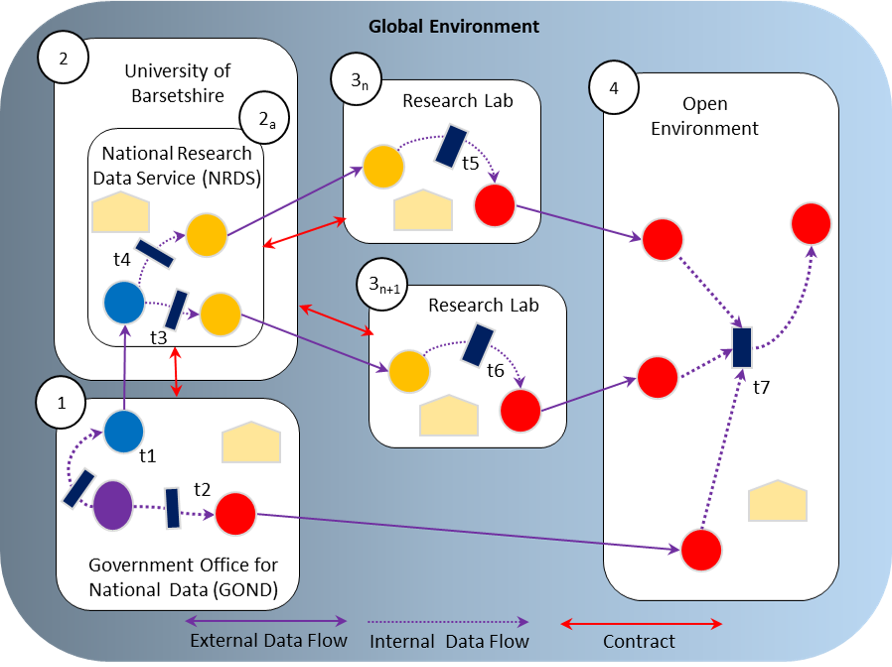
\includegraphics[width=\linewidth]{Picture1a.png}
\caption{A use case of data flows between and within multiple data environments. The red arrows indicate contractual agreements. The blue lines indicate data flow. Data environments are indicated by rounded rectangles, while data (circles), agents (pentagons) and activities (rectangles) are shown within their respective data environments. A circle represents a piece of data, a rectangle represent a process and a pentagon represents a user (in the data environment). The time for processing and sharing of data in the environments are labelled from \begin {math}t_1 \end{math} to \begin {math}t_7\end{math}.} \label{fig1}
\end{figure}
\begin{itemize}
\item Imagine that the Government Office for National Data (GOND) collects many types of national level datasets. For example, national census data, public healthcare data, birth-death related data, pupil data from schools, traffic data from the smart cities sensors, etc.
\item Part of GOND's remit is to make available some of that data for secondary research use. In service of this it shares versions of the national datasets that it holds with the National Research Data Service (NRDS).  
\item GOND also releases highly aggregated data into the public domain (by definition an open environment). 
\item The NRDS is part of University of Barsetshire. The NRDS's role is to acquire data from data holders, including GOND, under contract and then allow (and manage) access to those data under controlled conditions by researchers from research laboratories across the country.
\item The researchers carry out data analysis on GOND's data and then publish papers reporting on this analysis in the public domain. 
\item This data flow involves various loci of responsibility and control over the data sharing in and from the different environments.
\begin{itemize}
\item GOND has indirect responsibility and strategic control over the data release into the open environment (in the form of analytical output within publications). GOND  also has direct responsibility and control over the direct data released from its own environment into the public domain (in the form of aggregate statistics). 
\item NRDS's responsibility and control are different from GOND's, NRDS has direct and operational control over the data release from the output of publications.\footnote{See 
\end{itemize}
\end{itemize}

The sketch diagram of this use case is shown in Figure \ref{fig1}. Four focal data environments are part of global data environment. GOND, the University of Barestshire, and NRDS are represented as data environments 1, 2, and \begin{math}2_{a}\end{math}  respectively. The researchers and open environment are labelled with data environments \begin{math} 3_{n} \end{math} to \begin{math}3_{n+1} \end{math} and 4 respectively. As shown in Figure \ref{fig1}:
\begin{enumerate}
    \item Data starts in a GOND (1) data environment. At $t_1$, it is processed to make it compliant for sharing with (2), according to contractual obligations. At $t_2$, it is processed in a slightly different way to release publically (4).
    \item The data that is shared from GOND to the NRDS (2a), is similarly subjected to additional processing so that it can be shared with various research labs ($3_n,3_{n+1},....$).
    \item Each research lab analyzes the data according to their particular needs and research questions. The research labs wish to produce publications and research datasets for public consumption (4).
    \item One of the major goals of the ADF is to identify when data released by different organizations, that has been derived from the same original data, do not inadvertently disclose information.
\end{enumerate}


\subsection{ADF Requirements (using the GOND-NRDS use case)}
In order to understand the process of anonymisation decision-making in the GOND-NRDS use case a set of requirements have been identified. Based on these requirements, a data environment formalism will be created using W3C PROV data model (PROV-DM). PROV-DM is the conceptual data model and core part of W3C PROV that defines each term used to represent provenance information \cite{moreau2015rationale}.
The GOND-NRDS use case representation (i.e provenance graph) should be able to capture:

A specification of the requirements for representing data environments for the purposes of the ADF illustrated using the GOND-NRDS data situation is shown in table \ref{tab1}.

\begin{table}[!htbp]
 \setlength{\tabcolsep}{5pt}
\caption{Data environment representation requirements for GOND-NRDS use case.\label{tab1}}

%\bigskip
\centering
\begin{sideways}

\begin{tabular}{>{\raggedright\arraybackslash} p{0.2\linewidth} p{0.6\linewidth} p{0.75\linewidth}  }
\hline
\toprule
%\rowcolor{Gray}
\textbf{Requirement}  &  \textbf{Description}  &  \textbf{Example from the GOND-NRDS data situation} \\
%\hline
 \midrule
 \renewcommand{\arraystretch}{1}
Data Environment Construct &
The data environment construct defines a boundary state around data.  data controller, data processor,  data users,  data sharing, data situation, etc. 
%Data environment construct also defines the locus of control and locus of responsibility.
& GOND and NRDS are two closed data environments with different data and events.  \\
\midrule
Data Environments within Data Environments &
Sometimes an environment may contain other environments along with users, data, and processes. And data flows in the same organisation's sub units for processing, auditing, etc. & The NRDS data environment is contained within  the Barestshire university data environment and is an example of environments within environments. \\
\midrule
Attaching Attributes to Data Environments& 
For ADF to determine appropriate disclosure practices,  the purpose of data collection and type of data environment and any constraints and features (infrastructure and governance) of the data environment are attributes of the Data Environment.  &  GOND collects data from its partners for use and onward sharing because of legal obligations. The processing occurs in a restricted access data environment. On the other hand, the data shared through publication in the open environment is not restricted. \\   
\midrule
Relationships between Data Environments &
This describes the possible  relationship from data environment to another data environment & Within the NRDS, a Research Lab may have a specialized, secure processing environment which is owned and maintained by NRDS, but hosted for and used by the Research Lab. This is an example of a data environment with more complex relationships between data environment constructs than containment.\\
\midrule
Annotation to relational constructs & In order to reason over data environment interactions, controllers, processers, subjects, users, etc. it is important to allow the attachment of semantic meaning to the relationships among the constructs &  NRDS receive data from GOND and locally store it for onward to researcher. While in PROV  this can be labeled with \textit{prov:use} and \textit{prov:generated}. It doesn't represent the all of the required information needed by ADF to inform disclosure decisions. \\

Representation of agents, data and processes within a Data Environment & Agents include data controller, data processor, data users and data subjects. Data includes datasets, reports, etc. Processes include data extractions, sharing, storing, etc. &
  As GOND  and NRDS is a type of organisation data controller and processor. GOND is data controller with direct responsibility of his environment and indirect responsibility for NRDS environment. GOND is also a data processor, it generate datasets for NRDS and for an open environment. \\
\midrule
% \midrule
Contracts & 
An agreement or conditions to share, exchange and use data between the environments   &  GOND share data with NRDS based on the  contract between them. \\

\midrule

Access and control (Direct and Indirect)  &
A record of the existing access and control mechanisms over the data and services &  GOND has a data dissemination service/function that can be accessed/used by NRDS (based on some contract or data sharing agreements. GOND has also indirect control over the data release from the NRDS environment.  \\
\bottomrule   
\end{tabular}
\end{sideways}
    \end{table}





\section{Supporting Data Environments with W3C PROV} \label{sec:impl}
The W3C PROV data model structure and elements supports some of the data environment representation requirements. Because the elements of data environments can be mapped with PROV elements. PROV  properties can be used to represent the semantic relationship among the elements of data environment. However, there are some data environment specific requirements  that need extensions in PROV. In the following sub-sections we will explain how PROV can be applied to support data environment representation through four possible mechanisms.

\subsection{PROV Bundle}
In PROV, the bundle concept has some similarities to the data environment construct. %\todo{[ref]} \todo[color=green!40]{I didn't found any suitable reference. But from the explanation it is visible that they created bundle for similar purpose such as to capture provenance in multiple environments, so they can stitch it together. we can also remove this line if PROV baby looks ugly!\dSmiley}. 
The bundle itself is an entity which provides the provenance information of creation and modification of group of entities \cite{mckenna2019modelling}. 
%A bundle can also hold the provenance of other elements. 
For example a bundle can contain the entities, activities, agents, and the relationships between them. %This would enable us to represent the data controller, data processor, data subjects, and data users with the  \textit{PROV agent construct}. 
The  data, and data processes can be expressed with entities, and activities respectively. Bundles can also support entities with attributes. This can help us to add necessary metadata to the entities. 
%For example, essential means of data collection of GOND-NRDS use case can be expressed with additional metadata attachment to the entities inside the bundles. 
The excerpt view of the GOND-NRDS use case representation as supported by PROV bundles is shown in Figure \ref {fig:bundle}.

\begin{figure}[!htbp]
%\centering
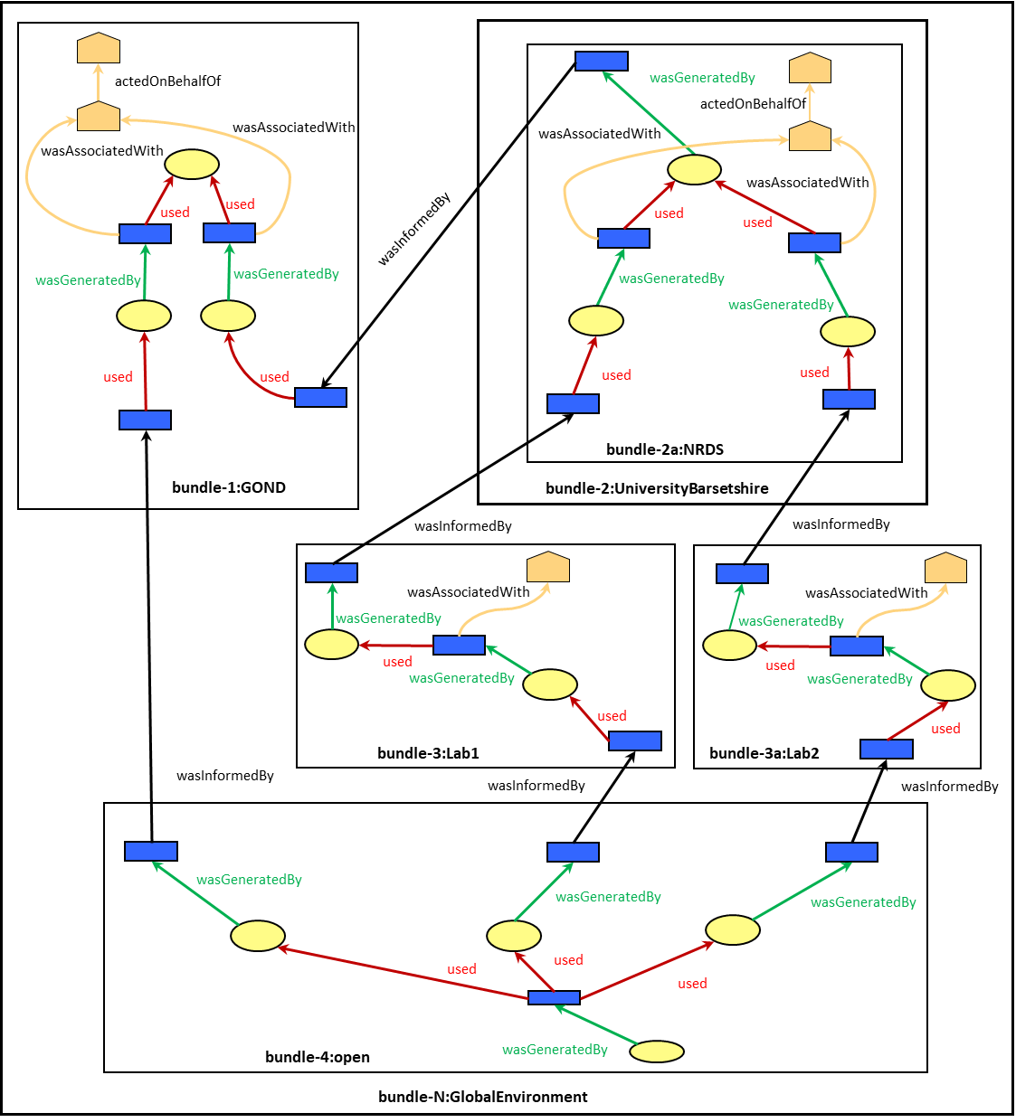
\includegraphics[width=\linewidth, height=8cm]{bundle.png}
\caption{A representation of the GOND-NRDS use case supported with PROV bundles} \label{fig:bundle}
\end{figure}

\subsection{Namespaces} \label{subsec:namespaces}
Namespaces are a Uniform Resource Identifier (URI). A provenance graph can contain many Namespaces. In PRVO-DM, the Namespace concept was inspired by the World Wide Web architecture and was designed to make objects interoperable across technologies and platforms \cite{moreau2015rationale}. 
PROV Namespace is a candidate for use as an identifier to capture the idea of multiple data environments (including data environments within data environments) and their associated entities, activities, agents, etc. 
By using Namespaces and  prefixes we can differentiate the representation of nested data environments and  can access related elements information through Namespace concatenating and de-concatenating. For example, we can refer the data environment of University  Baretshire and NRDS data environment (Note: In the use case NRDS data environment is a part of University Baretshire environment) as \textit{http://global-env.com/bu/ 
} and  \textit{http://global-env.com/bu/nrds/ 
} respectively. Additionally, we can also express the control mechanism over the data environments and its elements  with  Namespace feature. The visual representation of the GOND-NRDS use case  with the support of Namespaces and PROV constructs is shown in Figure \ref{fig:namespaces}.


\subsection{Namespaces with Support Structures} \label{subsec:namespacesplus}
While namespaces are powerful with respect to representing data environments boundaries, and what has occurred within a given data environment, and it's sub-data environments, namespaces themselves are not enough to satisfy all of the requirements identified within the use case. For instance, the attachment of additional attributes to the Data Environment itself and contracts between the data environments  cannot be accommodated. Additionally, relationships among namespaces beyond containment cannot be captured. For instance, it is possible with namespaces to distinguish that \textit{ http://www.nytimes.com}  data environment that contains a sub-data environments related to advertising functions, \textit{http://www.nytimes.com/ads}. However, within our use case, there is more than strict-hierarchical containment. On occasion, researchers from Research Labs have a specialized data analysis environment built-by, hosted-by and managed-by NRDS, but is considered an enclave of both NRDS and the Research Lab. In this case, namespaces do not capture enough information to represent this relationship.

To solve this, an additional set of structures would need to be created. For instance, a separate document which extends namespaces and allows attachment of attributes, could be utilized. 

\begin{figure}[!htbp]
%\centering
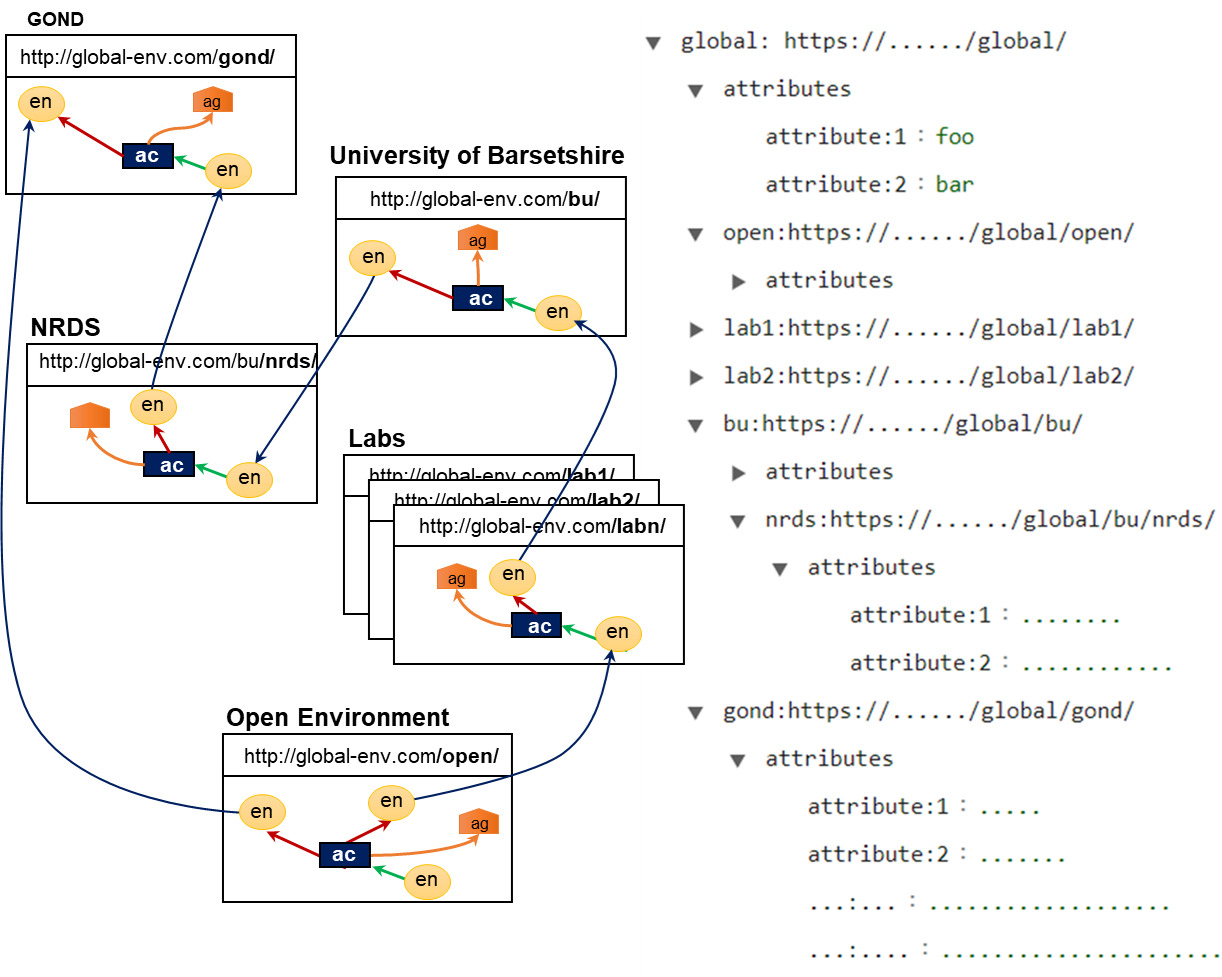
\includegraphics[width=\textwidth]{namespaces-2.png}
\caption{Illustration of the use of Namespaces to represent Data Environments: ag, ac, and en indicates agent, activity, and entity respectively; the right hand part  shows data environments with attribute attachment using Namespaces. Relationships across namespaces could be captured in the same manner. } \label{fig:namespaces}
\end{figure}

\subsection{Extended Bundles}   

W3C PROV constructs\footnote{The constructs are  structure and elements that are used to express the provenance of any object or thing.} were designed to be extensible \cite{moreau2015rationale}. PROV has already been extended to express the provenance of Big data security supervision \cite{gao2020big}, provenance access control \cite{missier2020abstracting}, data privacy protection based on GDPR using provenance \cite{davari2019access} and  managing mutable entities by adding reference derivations and checkpoints \cite{pimentel2018versioned}.
Similarly, we can extend the existing structure of PROV bundles in order to support and express the requirements of ADF  with better flexibility. For example, by extending we can attach  additional metadata with the bundle construct, which is necessary to define the types of  GOND-NRDS data environments. Another extension that we might need in PROV Bundles, is to support  nested data environments. if we consider the PROV bundle as a named set for the representation of data environment. On the other hand we can extend PROV by adding the new component (e.g. \textit{dataEnvironment}, \textit{endDataEnvironment}) for the data environment as a first class candidate and develop a new layer over the bundle structure. As a second step we could then build a mechanism to include attributes, entities, activities, agents, etc in each \textit{dataEnvironment}. In this approach, we can also reuse some of the existing features of bundles and entities. 

%comment by Age
\begin{comment}
Hang on here. Are there actually 2 things in this? 1) extend bundles and 2) make a new thing called data environments? If so, then we actually have 4 possible implementation strategies, and we need a new subsection to split them out (and analysis in that section, etc.  

However, I think what we actually have is a way to create data environments as first class citizens - by extending bundles. 

Could you comment on which it is?
\end{comment}

%comment by aslam
\begin{comment}
Actually this subsection previous title was "How PROV can be extended to support data environment" 

 possibly there are  three ways: 1) updated the bundle mechanism, 2) add data environment as a first class citizen

3) Namespaces with extra support of resources and documents as you described in paragraph starting with however... in section 3.2.  But I wondered  PROV community does not described Namespace likely Bundle, entity, etc. 

4.??? 
 can we leave this or for another paper?
\end{comment}
\begin{comment}
The first option might not be a suitable due to the nested data environments requirement. Because bundle neither supports bundle in a bundle and nor it provides the functionality of attributes attachment with the data environments. Therefore, the second option might take extra efforts but it will enables the comprehensive representation of data environments features. The requirement of similar  entities in multiple data environments  is relatively is a modelling and validation issue. This can be resolved as: 
\begin{itemize}
\item Like in object-oriented programming a variable with the same name can be declared in the class and multiple methods. However, the scope of the variable is limited to the class and methods in which it was declared. 
\item Similarly, there should be the support of multiple similar entities in multiple data environments within the same PROV document. And their scope should be limited to the data environment in which it is declared without explicitly indicating with prefixes.    
\end{itemize}

To resolve the issue of semantic annotation to properties two approaches can be possible. The first option is to  change non-semantic linking properties concepts and tags in the data model and change the labels for properties based on the application domain. The second option is to extend the mechanism of existing properties and introduce the "annotation to property" concept. We think that that the first option needs a continuous changes in the conceptual model and provenance document validation process because the properties concept and naming needs to be updated based on the use case. The second approach is suitable in the case of   data environment representation. Because all the existing properties and validation mechanism will be same, only the annotation attribute value will be updated based in the context of use case.
\end{comment}

\section{Comparative Analysis} \label{sec:analysis}

\subsection{Requirements Completeness}

To define the required provenance needed for the ADF in Section 4,  we analyze a healthcare-based ADF use-case (please refer Figure \ref{fig:usecase2})  in which:
\begin{itemize}
\item Data from clinical trials are generated at several participating centres data environment.
\item The data are uploaded electronically by the participating centres to a company called Medidata which offers an electronic data capture and management system for the pharmaceutical industry. 
\item PharComp, a European pharmaceutical business, extracts and downloads the clinical trial data from the Medidata database onto PharComp systems for analysis. 
\item PharComp share data with researchers, for researching on public health. 
\item Researchers publish their analysis in journal articles in the public domain. These data will not include information that identifies the patients, and additional steps are taken to safeguard the patients’ confidentiality.
\item  Explicit consent has been given by trial participants for secondary research use of anonymised data.
\end{itemize}
%The set of actions that has already occurred is retrospective provenance, and is shown in Figure 1 (using the W3C PROV standard [17e]).
%Because the data from EU citizens (amongst others) are being processed, the processing falls within the jurisdiction of GDPR and so that processing must either comply with the principles of GDPR and/or the data must be processed in a fashion which renders them anonymous information. 
%This creates both allowed (prescriptive) and not-allowed (proscriptive) actions.   is prescriptive provenance, and is shown in Figure 3.The proscriptive provenance is shown in Figure 2; the prescriptive provenance is shown in Figure 3.
%In our scenario, a research lab wishes to use PharComp’s anonymized data for further analysis and to publish a report in the public domain.  How does PharComp react to this new situation? This request by the research lab is prospective  provenance related to this action. Figure 4Figure 4 shows this provenance. % 
%Using this information, PharComp must be able to compare the desired actions, i.e., sharing a redacted version to the Research Lab, to defined “allowed” and “not allowed” actions. 




We use this Use Case to confirm that the requirements identified in Section \ref{sec:usecase} are correct (they are also seen in this healthcare use case) and complete (there are no additional requirements identified in the healthcare use case.

The \textbf{Data environment construct} is required to express the data situation within the environments of collection centers, Medidata, PharComp, research labs and open environment. As the data collection centers and research labs  contains sub-environments for various type of data collection and research protocol requirements, confirming the \textbf{“data environments within data environments”} requirement. In the use case, the Medidata and PharComp are type of private data environments and can be accessible to only authorized users and researchers. To express this type of and restriction to these data environments we need to \textbf{represent data, agents and processes}.  

Like the GOND-NRDS use case requirements, in this use case we need to \textbf{annotate the relationship constructs} between the data environments of collection centers and Medidata, where the data is collected and stored instead of data derivation/usage or generation. This will support the semantic meaning of relationship construct in the data provenance. Given the nature of the data collected for the pharmaceutical company, contracts specifying data collection, exchange and control exist (\textbf{contracts}). PharComp has  indirect control over the data release in the open environment in the form of publications and the researcher must follow the code and conduct given by the PharComp, this requirement can be represented with \textbf{access and control} category as mentioned in Table \ref{tab1}. 

Of the requirements presented in Table \ref{tab1} the \textbf{Relationship between data environments} is not not found in this use case, as there are no data environments with multiple institutional ownership and use. However, if the specific example contained an enclave in PharComp in which regulatory employees from a government could review specific data, this requirement would be met. There are no additional requirements that seem necessary to capture the provenance of data situation for ADF.
%\todo{Need a paragraph here, stating either There are No Additional REquirements for DE beyond Table 1. }
\begin{figure}
    \centering
    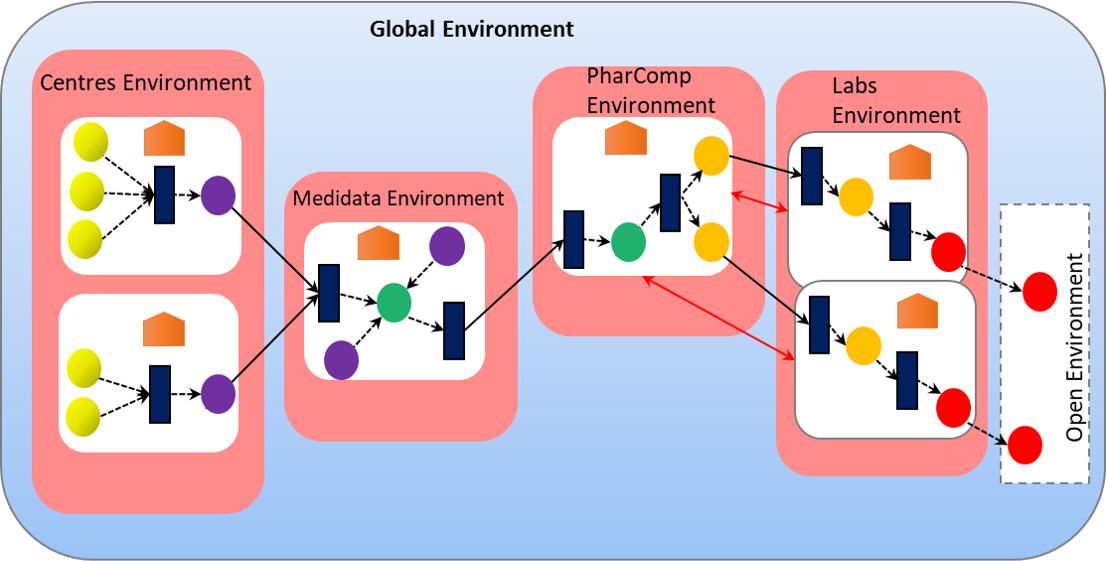
\includegraphics[width=\textwidth]{UseCase2.png}
    \caption{A second ADF Use Case with Data Environments: The red arrows indicate contractual agreements. The black lines indicate data flow. Data environments are indicated by rounded rectangles, A circle represents a piece of data, a rectangle represent a process and a pentagon represents a user in the respective data environment}
    \label{fig:usecase2}
\end{figure}
\subsection{Analysis of Implementation Approaches}
 In Section \ref{sec:usecase} we outlined an ADF Use Case that contains multiple data environments with agents who have a presence in multiple environments, and data that moves between them. Table \ref{tab1} contains the requirements for Data Environments drawn from the GOND-NRDS Use Case and verified by the PharComp Use Case. Table \ref{tab2} shows the data environment representation requirements and the ability of each of the implementation possibilities discussed in Section \ref{sec:impl} to meet those requirements. 

\begin{table}[!htbp]
 \caption{Use case requirements analysis, here Namespace + include attributes and PROV constructs}
  \label{tab2}
  %\centering
  \begin{tabular}{|p{5cm}|c|c|c|c|}
    \hline
    %\cline{2-4}
    \multirow{2}{*}{Representation requirements} &
    \multicolumn{4}{c|}{Support}   
     &  & Bundle & Namespace & Namespace+  &  Bundles+  \\
    \hline
    Data Environment Construct  & \checkmark & \checkmark & \checkmark & \checkmark \\
     \hline
    Data Environments within Data Environments  &  & \checkmark & \checkmark &\checkmark \\
     \hline
    Attaching Attributes to Data Environments &  &  & \checkmark &\checkmark \\
     \hline
     Relationship between Data Environments & \checkmark &  & \checkmark &\checkmark \\
     \hline
     Annotation to   relational constructs  &  &  & \checkmark &\checkmark \\
     
    % \hline
    % Data controller, processor, users and subjects & \checkmark &  & \checkmark &\checkmark \\
     
     
     %\hline
     %Representation of Agents, Data and Processes  & \checkmark & \checkmark  & \checkmark &\checkmark \\
     \hline
     Representation of agents, data and processes within DE  & \checkmark &  \checkmark & \checkmark &\checkmark \\
     \hline
     Contracts  & &  & \checkmark &\checkmark \\
    \hline
     
     Access and control & \checkmark & \checkmark & \checkmark &\checkmark \\
     
    \hline
  \end{tabular}
 
\end{table}

%\todo{The remainder of this until the next sub-section needs a re-write. The namespaces was not represented correctly, so future analysis needs to be smoothed.}
%\todo[color=green!40]{done}

The data environment nesting (i.e. data environments within data  environments) is one of the most important features. For example,  NRDS data environment is the part of University of Barestshire environment. However, with bundles we can not represent  nested data environments because PROV does not allow the nesting of bundles  \cite{moreau2015rationale}. On the other hand the data environments nesting  representation is  supported by Namespaces. For instance, a separate Namespace can be used to indicate a unique data environment.  Thus namespaces+ can also support nesting. This requirement is one of the driving features of bundles+.

The ability to attach attributes to a Data Environment are also one of the most important features of data environments for the ADF to analyse the data situation. Neither bundles or namespaces support attachment of attributes. For example, currently, we cannot express following  using PROV bundle.  \\
 \begin{math}bundle (EX-A:GOND, [prov:envType ="Government", prov:accessType="Restricted") \end{math}. \\
However, the additional structures provided in Namespace+ allows attributes to be maintained with the namespace information. Bundles+ is a much more elegant option, by using the W3C PROVs standard of attaching attributes to other object types, and expanding that notion to bundles+.
 As we have observed in the GOND-NRDS use case (please refer Figure \ref{fig1}), the GOND data environment contains the representation of  collected, processed and shared data along with the data processes, agents, and contracts (i.e. contract with the NRDS), and IT (Information Technology) infrastructure and services. In order to create the provenance graph for GOND data environment representation, the relationship among these elements are supported with PROV properties. For example  \textit{ wasGeneratedBy (entity\_id , activity\_id)}, and \textit{used(activity\_id, entity\_id)} properties are used to represent the relationship between the GOND collected data and process over the data for generating the new dataset for NRDS. Bundles and Namespaces naturally support the representation of agents, processes and entitities using native W3C PROV concepts. On the other hand, supporting additional metadata such as annotation with the relationship constructs is not fully supported in PROV. However, this  can be managed  by attaching additional attributes with the relationship construct as done  in  \cite{pimentel2018versioned} for tracking the changes in entities over the time. We believe that to represent the true meaning of relationship among the data environment elements attaching annotation is necessary. Attaching annotation will also be helpful in selecting an appropriate information disclosure process. %The  data environment as a first class citizen will supports this requirements for GOND-NRDS use case. The GOND-NRDS data, contracts, and data events are supported by Bundles, Namespaces plus, and PROV extension.
 The  PROV extension with extended bundles will supports this requirements for the GOND-NRDS and PharComp use cases. The GOND-NRDS  and PharComp  contracts are  supported by Bundles+  and Namespaces+.
 Moreover, access  control representation requirement is supported by all four constructs.  


%The Bundles construct can be discarded almost immediately. Bundles cannot be nested, and was designed not to support the scoping mechanism of identifiers \cite{moreau2015rationale}. Therefore, the bundle cannot support the requirement of Data Environments in Data %Environments for GOND-NRDS use case. 




     


\section{Related Work} \label{sec:relwork}

%\subsection{Extending W3C PROV}
The W3C PROV has been used to capture provenance to protect data subjects privacy, and security of data. A W3C PROV based provenance model has been proposed by Benjamin et al. \cite{ujcich2018provenance} that uses the PROV data model ontology and data protection ontology to express the provenance for compliance of the European Union (EU) General Data Protection Regulation (GDPR). The Agent, Activity, and Entity classes from the PROV ontology were extended with sub-classes to express the provenance for GDPR compliance. For example, \textit{Subject}, \textit{Controller}, \textit{Processor}, and \textit{Supervising-Authority} sub-classes were introduced within the agent class. The Activity class was extended with  two additional sub-classes: \textit{Process} and \textit{Justify}. Similarly, the Entity class was extended with three sub-classes:  \textit{PersonalData}, \textit{Request} and \textit{Justification}. The relationships among the classes were expressed with PROV properties. Both of the ADF examples presented in this work fall under GDPR regulations, and the extensions introduced in Benjamin et al. \cite{ujcich2018provenance} would facilitate some of the more general requirements of \textbf{Representation of agents, data and processes}and \textbf{contracts} within Data Environments.

To support  provenance of mutable values by time-versioning entities,  a PROV extension has been developed by adding the reference sharing and checkpoints feature \cite{pimentel2018versioned}. These features were built on top of  PROV events that track a version of and object or entity through changes on generation events (i.e. \textit{prov:Generation}) and access in  usage events (i.e. \textit{prov:used  }). The checkpoint attributes were used with the PROV entities, activities, relationship properties for tagging and tracking of changes in the entities over the time period. For this purpose, two Namespaces (i.e. version and script) were created to support the checkpoints mechanism. The version and script Namespaces were used for general PROV extension concepts and specific script concepts. However, this approach increases the extra overhead for querying the provenance graph due to folding and unfolding for adding the checkpoints.  

% \subsection{Using provenance to protect data and systems}
% Data provenance is  applied to detecting intrusion and faults in the operating system kernel environments. For this purpose the CamFlow \cite{pasquier2017practical}  was developed with the notion of "whole system provenance" that
%  detect  attacks by the intruders in the Linux Kernel.  CamFlow captures the provenance features by using  Linux Security Modules (LSM) and NetFilter (NF) hooks. In these features it is recorded that how the information is exchanged through system calls at point in time and in shared state. %For representing the provenance features, the CamFlow's authors have extended W3C PROV Data Model (PROV-DM) \cite{PROV-DM15}.
%  In the captured provenance  the kernel objects such as files, messages, packets, network addresses,  inode attributes, exec parameters have been represented as entities. And system calls and operation processes (e.g. read, write) were represented as activities. For CamFlow's proof of concept, two provenance graphs containing  system state with correct behaviour  and incorrect behaviour were generated in the cloud streaming environment. And finally both provenance graphs were matched through sliding windows technique for the detection of attacks in the streaming. \todo{Aslam, please go look up CamFlow. It may not be w3c, but it is provenance. They (and a few other groups working with them) are using provenance to detect intrusion detection attacks.} \todo[color=green!40]{updated,---   }   

In order to supervise  security of big data streaming, the W3C PROV data model has been extended with a new relationship properties \cite{gao2020big}. These properties focus on  collecting the provenance information about the  data operations inside and outside of big data clusters. It represents the data interaction flow between the clusters. The harvested relationship provenance information of the graph is analysed for the detection of anomalies in the data. The anomaly detection and reasoning mechanism checks any inconsistency among the nodes and edges. To capturing the features for verifying the originality and source of data  received from sensors and edge cloud devices, the data situation can be modelled based on the data provenance . For this purpose, authors \cite{pahl2018architecture}, have used the W3C PROV data model along with the blockchain technology to implement the trust analysis platform. Which perform the trusted orchestration of devices in the edge  IoT environment. Additionally, the W3C PROV has been used to protect the data provenance content that are sensitive  and subject to disclosure control \cite{missier2020abstracting}, modelling the threat of attack to supply chain electronic management system \cite{halak2021cist}, and detection of bottlenecks in the system by analysing the patterns in the provenance graph \cite{boutamina2018bottleneck}.


\section{Discussion} \label{sec:discussion }

Continuing this work, for its application to the ADF would require substantial updates to the W3C PROV tools that are currently available, no matter which of the two solutions is chosen. However, considering that the Bundles+ solution uses W3C PROV concepts, and merely applies them to Bundles, as opposed to adding new concepts and structures to namespaces, we consider the Bundles+ option to be more elegant. To this end, we identify the modifications to W3C PROV support code in order to be fully integrated.

\subsection{Data Environment Representation Document Generation}
Currently, to generate a PROV based data environment representation document by using the python library, the  prov module is imported \textit{(e.g. import prov.model as prov)} in the source code. After that, the PROV document instance \textit{(e.g. ProvDocument())} is created. This instance provides the methods for creating a PROV document. For example, the  \textit{add\_namespace()} method is used to assigns a prefix and URI to the PROV document and elements;  entity(), activity(), and agent() methods are used to create the entity, activity, and agent respectively.  The \textit{ProvDocument()} instance also initializes the bundle class instance. Subsequently, the bundle instance provides the methods to add the entity, activity, etc within bundles. We need to add a new method in the \textit{ProvDocument} class that provides the instance of the \textit{ extended bundle} class. The  \textit{bundle class} class instance should contain the method for entity, activity, agent and linking properties as well as recursive method for the \textit{bundlePlus}. For example, \textit{bundlePlus.entity(), bundlePlus.activity(), bundlePlus.agent(), bundlePlus.bundle()}. We also need a new method to attach attributes to the data environment. At the last the method \textit{get\_provn()}  of \textit{ProvDocument()}  class that generate provenance document representation in  should be updated accordingly. 

\subsection{Validation of Data Environment Representation}
Currently, the source code for PROV validation is not openly available. However, the source codes for the SEIS-PROV’s\footnote{SEIS-PROV is a domain specific extension based on the W3C PROV data model, used in the seismological data processing. This extension defines a new namespace with entities, activities and attributes in the context of seismology.}   document validation is openly available at \cite{SEISPROV}. The SEIS-PROV validation mechanism is implemented in python. Using this validation tool as an exemplar, to validate the representation that includes the data environments in data environments, the prov document should include a formalism for data environments:
\begin{math}
[d_i=I_i \cup d_1,....,[d_n=I_n \cup  d_{n-1}] 
\end{math}
where  n is number of data environments and prov elements instances, I is the top level prov element instance and d is the data environment instance.The value of i will be between 0 and n. 

The PROV validation mechanism has two parts: inference and constraints. The inferencing  deals with the fixing of missing information based on the definition of the element defined in the PROV data model. The constraint component includes the checking mechanism that deals with uniqueness, ordering, impossibility and typing. Impossibility checks prohibited patterns, while typing constraints check the type of identifier when it is used in relations.    
Inferencing should be performed over the document, and the elements should be categorised as per the definition. 
For example, similar entities in two different data environments might be categorised according to the prefixes of definition or prefixes over the data environment.
     
\subsection{Translation and Visualisation} 
In order to share the data environment representation with other stakeholders it might be possible that they needs the transformation of representation from PROV-N to other formats (e.g. json, provx, turtle, trig, svg, rdf, xml) and vice versa. %Therefore, for the addition of \textit{dataEnvironment} as a first class citizen and extension in PROV bundles, the existing translation and visualisation mechanism will also needs substantial changes.
Therefore, due to the extension in PROV bundles, the existing translation and visualisation mechanism will also needs substantial changes.
%uncomplete 
Our goal is to incorporate the support for data envrinemnt representation in PROV python implementation. The PROV python implementation provides a PROV serialisation module \cite{provpythonpkg} that provides various classes to transform PROV document from one format to another format. For example, \textit{ProvJSONSerializer, ProvRDFSerializer, ProvNSerializer, ProvXMLSerializer} provides the implementation to translate PROV in JSON, RDF, prov notation and XML formats respectively. All of these serialisation classes needs substantial changes  

For graphical visualisation of provenance statements, PROV python implementation is using three open source libraries pydot \cite{pydot2021}, Graphviz \cite{ellson2001graphviz}, and DOT language \cite{gansner2006drawing} in \textit{prov.dot} module. Moreover, the \textit{prov.dot} module also needs substantial changes in \textit{prov\_to\_dot()},  \textit{ \_bundle\_to\_dot()},      \textit{\_attach\_attribute \_annotation()},  etc
methods that translate the  provenance statements into visualization graphs. 
These methods needs considerable updations along with additional methods  to support the graphical visualization of  data situation among the data environments. 
\section{Conclusions and Future Work} \label{sec:concl}

In this work, we consider a new application of provenance: to assist in determining the correct sharing mechanisms for data exchanged across organizations and environments. To this end, we introduce the Anonymization Decision Framework (ADF) which is used to manually reason over data flows and data exchange requirements. Through analysis of the ADF, how it is applied, and the information required to make such decisions, we have identified how provenance can be utilized in the future to create more automated decisions.

 In order to express the data situation, the data environments elements: other data, data agents, governance processes, infrastructure have been identified from a real world use case and mapped with W3C PROV elements: entities, bundles, activities, and agents. Further, to fully express the features of data environments for exploiting the ADF based machine enabled reasoning, we observed that the existing PROV constructs are not sufficient and need an extension. 
 
To this end, we analyze how data environments can be represented within the W3C PROV. We identify four different mechanisms within the W3C PROV, and evaluate each with respect to trade-offs of cost, maintenance and suitability for ADF. While two obviously does not pass muster, the other two are viable solutions, with one that utilizes existing W3C PROV structures and require an additional management, and the  second needs an extension.
\bibliographystyle{unsrt}
\bibliography{references.bib}
\end{document}



%\begin{thebibliography}{8}
%\bibitem{ref_article1}
%Author, F.: Article title. Journal \textbf{2}(5), 99--110 (2016)

%\bibitem{ref_lncs1}
%Author, F., Author, S.: Title of a proceedings paper. In: Editor,
%F., Editor, S. (eds.) CONFERENCE 2016, LNCS, vol. 9999, pp. 1--13.
%Springer, Heidelberg (2016). \doi{10.10007/1234567890}

%\bibitem{ref_book1}
%Author, F., Author, S., Author, T.: Book title. 2nd edn. Publisher,
%Location (1999)

%\bibitem{ref_proc1}
%Author, A.-B.: Contribution title. In: 9th International Proceedings
%on Proceedings, pp. 1--2. Publisher, Location (2010)

%\bibitem{ref_url1}
%LNCS Homepage, \url{http://www.springer.com/lncs}. Last accessed 4
%Oct 2017
%\end{thebibliography}